\documentclass{article}
\usepackage{graphicx} % Required for inserting images
\usepackage[export]{adjustbox}
\usepackage{listings}
\usepackage{color}

\definecolor{dkgreen}{rgb}{0,0.6,0}
\definecolor{gray}{rgb}{0.5,0.5,0.5}
\definecolor{mauve}{rgb}{0.58,0,0.82}

\lstset{
frame=tb,
language=C,
aboveskip=3mm,
belowskip=3mm,
showstringspaces=false,
columns=flexible,
basicstyle={\small\ttfamily},
numbers=none,
numberstyle=\tiny\color{gray},
keywordstyle=\color{blue},
commentstyle=\color{dkgreen},
stringstyle=\color{mauve},
breaklines=true,
breakatwhitespace=true,
tabsize=3
}

\title{Algoritmo parallelo per la somma di N numeri}
\author{Puggioni Riccardo,Regina Riccardo,Trotti Francesco }
\date{October 2023}

\begin{document}

\maketitle

\section{Introduzione al problema}
\subsection{Somma di N numeri}
    L'algoritmo per la somma di N numeri fa parte di quei problemi
    il cui approccio alla risoluzione è detto di "riduzione".
    Parallelizzare Questo tipo di algoritmi può essere particolarmente insidioso:
    quando si sommano N numeri quello che si fa è eseguire N-1
    operazioni di somma; il nostro obiettivo è cercare di parallelizzare le operazioni di somma eseguendole su più processori diversi diminuendo in questo modo i passi temporali necessari alla risoluzione del problema.

    Ciò che però ci preme è non solo di risolvere il problema
    dato utilizzando un algoritmo parallelo, ma cercare di sfruttare al meglio il nostro ambiente di calcolo.
\subsection{Approccio alla risoluzione del problema dato}

   

    Andiamo dunque ad implementare la strategia di parallelizzazione in linguaggio C utilizzando una libreria per il "message passing" in un sistema MIMD (la libreria MPI).
    \\
    L'idea principale per la risoluzione del problema è di dividere l' array fra i vari processori.
    Fatto questo, ogni processore dovrà calcolare la somma parziale degli elementi del suo sotto-array
    e si dovranno poi ricostruire le varie somme parziali in maniera opportuna per ottenere la soluzione finale.\\
    \begin{figure}[!htbp]
        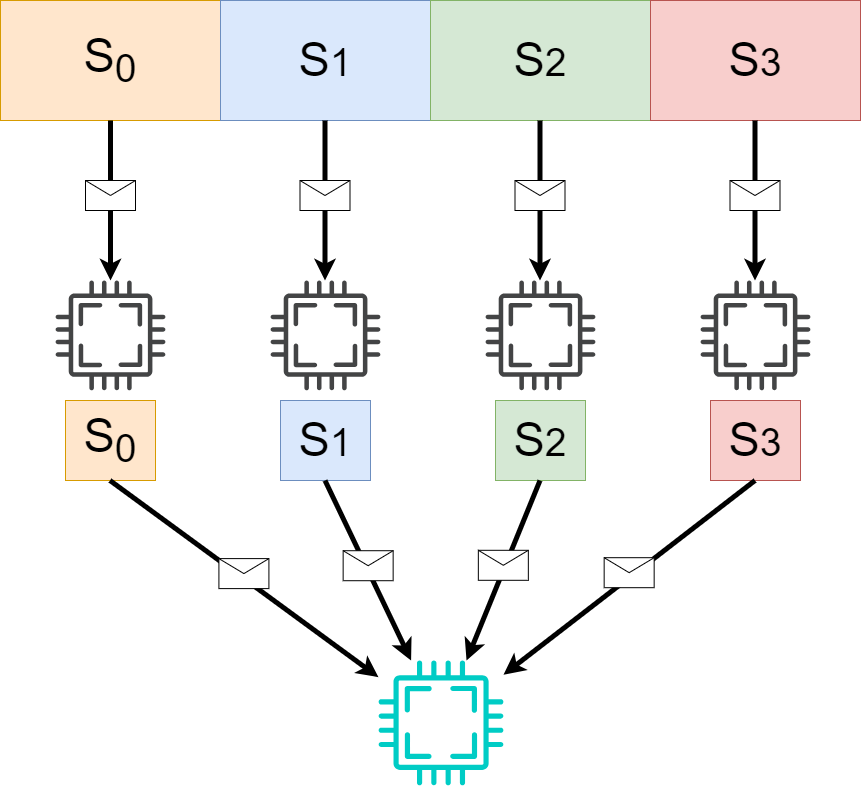
\includegraphics[width=0.3\linewidth,center]{divisione_array.drawio.png}
        \caption{Divisione dell array in parti}
        \label{fig:enter-label}
    \end{figure}  
    
    Ipotizziamo ora di voler implementare il nostro algoritmo, individuiamo tre passi fondamentali:
    \begin{enumerate}
        \item dividiamo l'array in più parti e assegnamo ogni parte a un processore.
        \item ogni processore esegue la propria somma parziale.
        \item si ricombinano le soluzioni parziali e si ottiene la soluzione finale.
    \end{enumerate}

    Facendo in questo modo possiamo così eseguire più somme concorrentemente, e il nostro algoritmo sarà di conseguenza più rapido.\\
    Una prima idea sarebbe dunque quella di prendere la dimensione dell array e di dividerla per il numero dei processori utilizzati: in questo modo otteniamo (all'incirca) il numero di elementi che ogni sotto-array dovrà contenere (a meno dei resti della divisione che si dovranno poi gestire nell'implementazione).

    \begin{figure}[!htbp]
        \centering
        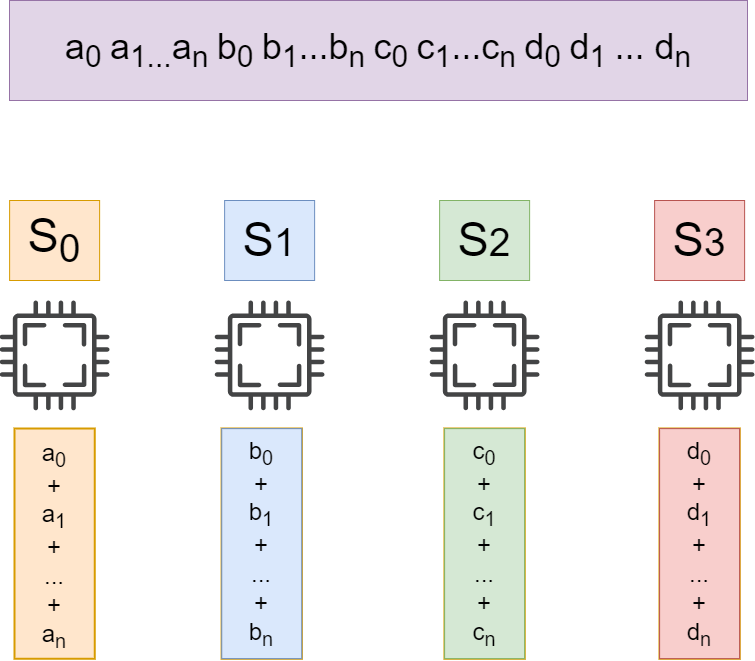
\includegraphics[width=0.6\linewidth]{somme_parziali.drawio (1).png}
        \caption{Ogni processore esegue la sua somma}
        \label{fig:enter-label}
    \end{figure}

    Una volta eseguita la distribuzione dei dati fra i vari processori passiamo all' algoritmo vero e proprio: ogni processore non deve far altro che sommare gli elementi del proprio sotto-array producendo le somme parziali.\\
    

\subsection{Strategie di comunicazione}
 Bisogna ora capire il modo in cui queste somme devono essere ricombinate, a tal scopo analizziamo tre possibili modalità di procedere:
\subsubsection{Strategia I}
    La prima strategia è la più intuitiva.
    Consiste nel prendere le varie somme parziali e mandarle tutte ad un processore specifico: sarà lui che eseguirà la somma delle varie somme parziali e che otterrà la soluzione finale al problema.
    Tuttavia seppur questa implementazione sia molto semplice (e funzionante in ogni caso), non rappresenta sempre la scelta più performante in quanto una volta che inviamo al processore scelto tutte le somme parziali, questo eseguirà la somme rimanenti in maniera sequenziale, mentre gli altri processori non saranno utilizzati affatto. La somma finale sarà presente dunque soltanto nella memoria del processore scelto per il calcolo finale.\\
    Come si evince anche dalla figura, ci saranno delle somme che potevano essere parallelizzate ulteriormente...(in date condizioni). 

    \begin{figure}
        \centering
        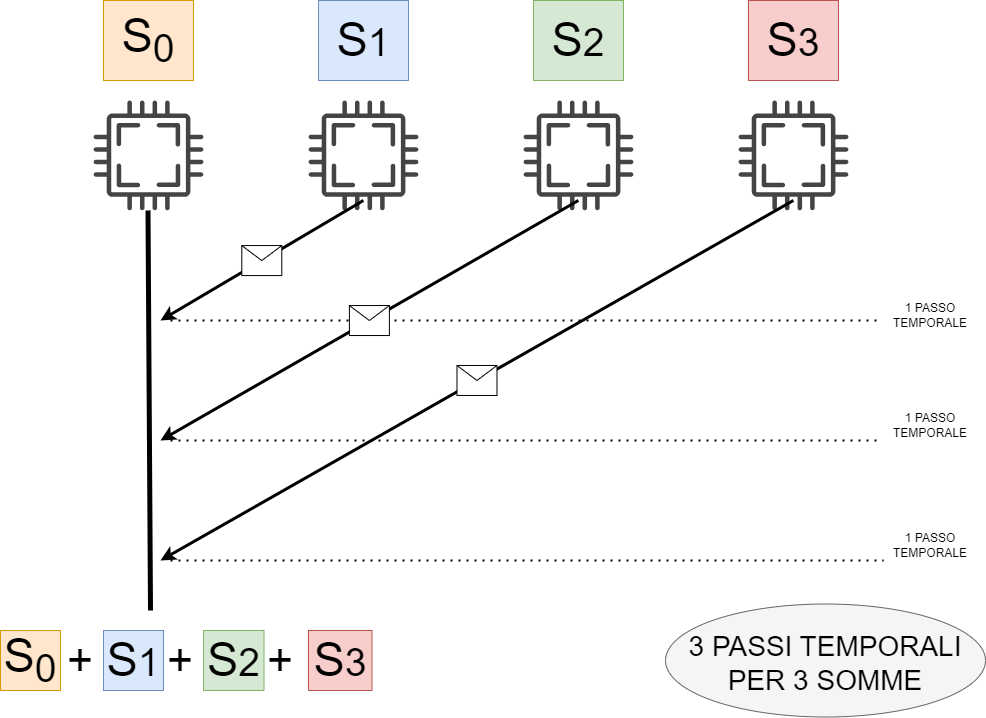
\includegraphics[width=1\linewidth]{strategia_I.drawio.png}
        \caption{Ognuno invia ad un processore}
        \label{fig:enter-label}
    \end{figure}
\subsubsection{Strategia II}
    La seconda strategia differisce dalla prima poichè i processori si dividono in coppie: uno dei due invia all'altro la propria somma parziale e l'altro ricevendo i dati aggiorna la propria somma.
    Alla fine l'ultima coppia aggiornerà l'ultima somma parziale ottenendo il risultato finale.
    L'ultimo processore che riceverà conterrà la somma totale.\\
    Tuttavia ci accorgiamo subito che, in una prima analisi preliminare, l'implementazione di questa strategia fa sicuramente sì che si risparmino passi temporali preziosi, ma può essere applicata soltanto se il numero dei processori in gioco è una potenza di due. Infatti non potrei dividere i processori sempre in coppie se questa condizione non fosse soddisfatta.
\begin{figure}
    \centering
    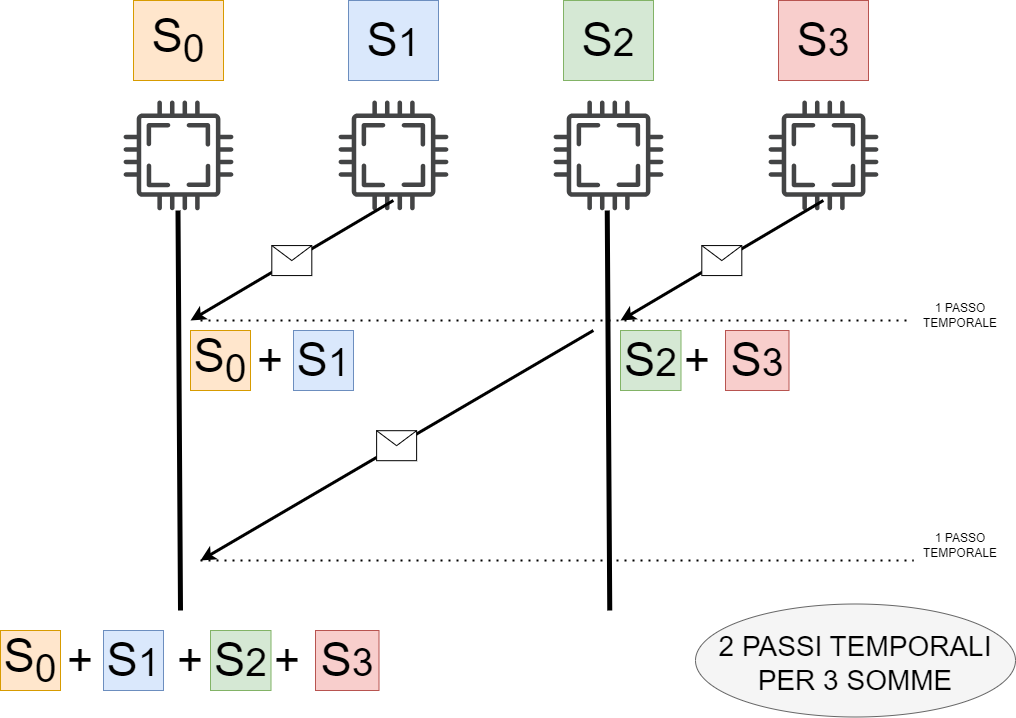
\includegraphics[width=1\linewidth]{strategia_II.drawio.png}
    \caption{In coppie (uno manda e uno riceve)}
    \label{fig:enter-label}
\end{figure}
\subsubsection{Strategia III}
    La terza strategia è simile alla seconda: divido sempre in processori in coppia.
    Tuttavia questa volta ogni coppia di processori si invia a vicenda la propria somma parziale e aggiornano entrambi la loro somma. Alla fine saranno tutti i processori ad avere il risultato finale in memoria.Tuttavia i passi temporali che risparmiamo sono gli stessi della strategia due, la principale differenza è infatti nel solo fatto che tutti i processori alla fine avranno la somma totale.
    \begin{figure}[!h tbp]
        \centering
        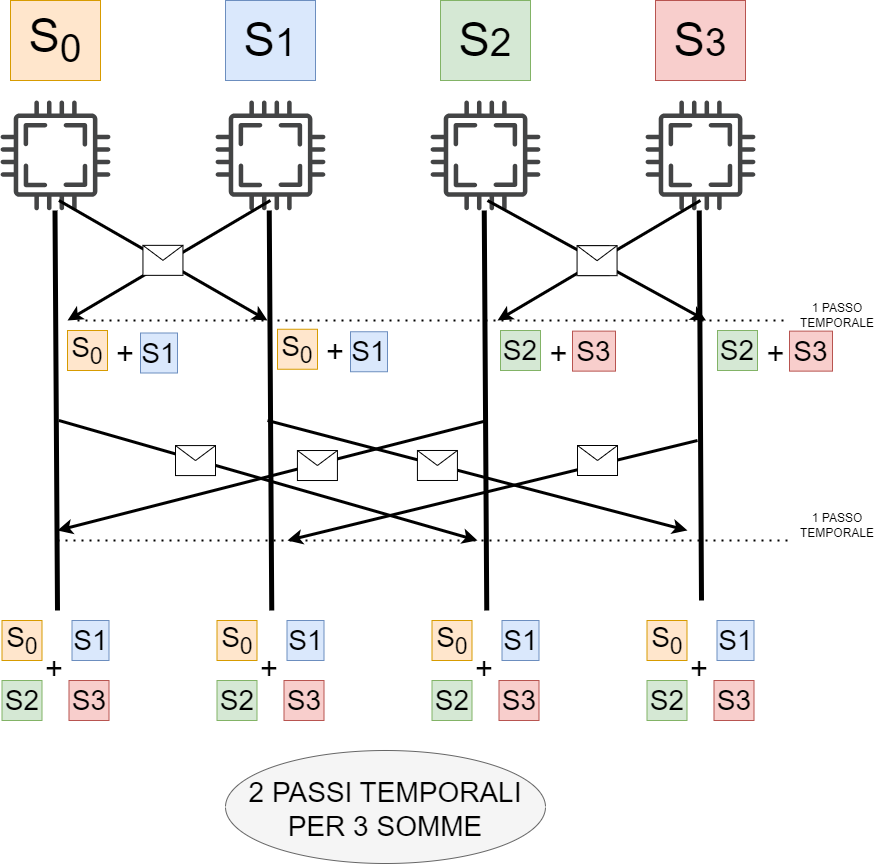
\includegraphics[width=1\linewidth]{strategia_III.drawio.png}
        \caption{In coppie (entrambi mandano e ricevono)}
        \label{fig:enter-label}
    \end{figure}
\clearpage
\section{Implementazione dell'algoritmo}
\subsection{Header file richiamati}
\begin{lstlisting}
#include <stdlib.h>
#include <stdio.h>
#include "mpi.h"
\end{lstlisting}

\subsection{Dichiarazioni}
\begin{lstlisting}
int main(int argc,char *argv[]){
    
    int pid,n_processi;
    int strategy;
    int n_locale,rest;
    int *array_locale;
    int tmp,start,tag;

    MPI_Status status;

    MPI_Init(&argc,&argv);

    MPI_Comm_rank(MPI_COMM_WORLD,&pid);
    MPI_Comm_size(MPI_COMM_WORLD,&n_processi);

    int *x;
    int n;

    if(pid==0){
        //leggi i dati dall input (n e x)
        FILE *fp;
        fp=fopen("/homes/DMA/PDC/2024/TRTFNC03B/sum/sum.txt","r");

        fscanf(fp,"%d ",&n);

        x=malloc(n*sizeof(int));
        int i;
    for(i=0;i<n;i++){
        fscanf(fp,"%d ",&x[i]);
    }
        fclose(fp);
    }

    MPI_Bcast(&n,1,MPI_INT,0,MPI_COMM_WORLD);

    n_locale=n/n_processi; //dividiamo la dimensione dell array per il numero di processi 
    rest=n%n_processi;     //e gestiamo il resto in modo da ottenere la dimensione
    if(pid<rest){           // del sottoarray per ogni processo.
        n_locale++;
    }

    if(pid==0){
        array_locale=x;
        tmp=n_locale;
        start=0;
        int i;
	    for(i=1;i<n_processi;i++){    //spezziamo l array in piu parti e mandiamo
            start=start+tmp;              //ad ogni processo la sua parte.
            tag=22+i;
            if(i==rest) {	
                tmp--;
		    }
            MPI_Send(&x[start],tmp,MPI_INT,i,tag,MPI_COMM_WORLD);
        }
    }
    else{
        tag=22+pid;
        array_locale=malloc(n_locale*sizeof(int));
	    MPI_Recv(array_locale,n_locale,MPI_INT,0,tag,MPI_COMM_WORLD,&status);  
        //i processi ricevono la propria parte.
    }

    //tutti i processori eseguono poi la propria somma parziale:
    int somma_parziale=0;
    int i;
	for(i=0;i<n_locale;i++) {
       	somma_parziale = somma_parziale + array_locale[i];
	}

    //Strategia di comunicazione 2
    int somma_totale = 0;
    for (i = 0; i < log2(n_processi); i++) {
        if (pid % pow(2,i+1) == 0) {
            MPI_Recv(&somma_totale, 1, MPI_Int, pid+pow(2,i), tag, MPI_COMM_WORLD, &status);
            MPI_Send(&somma_parziale, 1, MPI_Int, pid+pow(2,i), tag, MPI_COMM_WORLD, &status);
        } else {
            MPI_Recv(&somma_totale, 1, MPI_Int, pid - pow(2,i), tag, MPI_COMM_WORLD, &status);
            MPI_Send(&somma_parziale, 1, MPI_Int, pid - pow(2,i), tag, MPI_COMM_WORLD, &status);
        }
    }

    if(pid==0) printf("somma=%d\n",somma_totale);

    MPI_Finalize();
}
\end{lstlisting}

\section{Analisi dei tempi}
Nell' approccio a calcolare il tempo di esecuzione di un algoritmo parallelo, la grandezza note come complessità di tempo (utile nell analisi del tempo di esecuzione di un algoritmo sequenziale) diventa inutilizzabile.\\
In un algoritmo parallelo il numero delle operazioni non coincide più con il numero dei passi temporali, di conseguenza si introducono nuove grandezze al fine di realizzare un analisi degli algoritmi paralleli. Nel caso particolare in cui si debbano sommare N numeri, il numero di operazioni di somma da effettuare è N-1.

In un ambiente di calcolo parallelo con P che indica il numero di processori, un problema che si risolve in un tempo T ci darà che, \textit{T(P)} è il \textit{tempo di esecuzione su p processori}. Il problema si svolgerà idealmente in $\frac{T}{P}$, ma, come vedremo, potremmo solo cercare di avvicinarci a tale rapporto. 

\subsection{Tempo di esecuzione}
In un ambiente di calcolo parallelo con P che indica il numero di processori, un problema che si risolve in un tempo T ci darà che, \textit{T(P)} è il \textit{tempo di esecuzione su p processori}. Il problema si svolgerà idealmente in $\frac{T}{P}$, ma, come vedremo, potremmo solo cercare di avvicinarci a tale rapporto.\\
Il numero di operazioni dell'algoritmo di somma parallela è:
$$T(p)=(\frac{n}{p}-1 + \log_2(p))t_{calc}$$

\subsection{Speed-up, Efficienza, Overhead}

Lo \textbf{Speed- up} misura la riduzione del tempo di esecuzione rispetto all'algoritmo su 1 processore ed è definito dal rapporto:
$$ S(P) = \frac{T(1)}{T(P)} $$ 

In seguito a semplici passi algebrici, definiamo l'Overhead come
$$O_h(p) = pT(p) - T(1)$$
Esso è idealmente nullo e misura la 

Lo speed-up che noi vogliamo ottenere è sempre più prossimo a quello che si definisce come speed-up ideale.
Lo speed-up più vicino a quello ideale è quello nel caso di 2 processori. Ma sappiamo che non è la situazione più efficiente

Per poter misurare se e quanto è stato "sfruttato" il calcolatore parallelo dobbiamo calcolare l'efficienza del nostro algoritmo.
Si definisce \textbf{efficienza} il rapporto che risulta essere: $$ E(p) = \frac{S(p)}{p} $$\\
In generale ci risulta che: $$ E(p) < 1 = \frac{S_{ideale}(p)}{p} = E_{ideale} $$\\


\subsection{Dati empirici}
L'algoritmo è stato testato in più condizioni e secondo i parametri precedentemente descritti.

Avendo fissato ad un milione la dimensione del problema ed avendo fatto variare il numero di processori da 1 a 8, tenendo conto esclusivamente delle potenze di 2, sono stati ottenuti i seguenti risultati:
RISULTATI

Visualizziamo la curva, confrontandola all'andamento dello speed-up ideale:
GRAFICO

QUI PARLO DELL'OVERHEAD

QUI PARLO DELL'EFFICIENZA

Per non far degradare lo speedup, possiamo sfruttare il concetto di isoefficienza: per sfruttare l'aumento di processori, dobbiamo aumentare anche la dimensione del problema. Il coefficiente di aumento della dimensione non è costante, ma va opportunamente calcolato. Nel nostro caso, l'isoefficienza è la seguente:
$$I(n_{0}, p_{0}, p_{1}) = n_0\frac{p_{1} log_{2} p_{1}}{p_{0} log_{2} p_{0}} = n_1$$
dove $n_0$ è la dimensione del problema per $p_0$ processori, $n_1$ è la dimensione che vogliamo calcolare per $p_1$ processori.

Calcolati i coefficienti opportuni, i risultati sono stati i seguenti:
RISULTATI

GRAFICO

\end{document}
